% vim: tw=80

\chapter{Introduction}

Modern particle physics is driven by the desire to answer the questions about the
fundamental constituents of matter and the principles of interaction between
them. High-energy collisions of particles and the analysis of their
scattering byproducts are an optimal method to gain deep insights into the
fundamental principles of our universe. 

In the endeavor to reach highest energies in order to produce very rare particles and
search for new physics, the particle accelerators became ever bigger and more
complex culminating in the construction of the Large Hadron Collider (LHC).

In the LHC, bunches of protons are accelerated to high energies and brought to
collision. The constituents of the protons, quarks and gluons, interact and can
produce a plethora of new particles. Their decay products are detected and
measured precisely in huge particle detectors installed at the LHC. The CMS
detector used in this thesis is one of the two main detectors at the LHC.

Quarks and gluons manifest themselves as streams of collimated particles in the
detector and are clustered into so-called particle jets. The measurement of
events containing two such jets with large transverse momenta, dijet events,
allow for rigorous tests of predictions of Quantum Chromodynamics (QCD) and can
subsequently also be exploited to gain a better understanding of the proton structure
and to determine the strong coupling constant.

Dijet observables are best suited for proton structure studies as they can be
measured precisely and perturbative QCD predictions exist at next-to-leading
order accuracy. The proton structure is described by parton distribution
functions (PDFs) which give the probability to find a quark or gluon at a scale
$Q$ with a fractional momentum $x$ of the proton. The $x$ dependence is not
predicted by QCD but has to be parametrized and determined from fits to
experimental data.

In this thesis, a triple-differential measurement of dijet cross sections at the
LHC is explored for the first time. The theoretical considerations which led to
the chosen set of observables are introduced. Fig.~\ref{fig:intro_ybys_hint}
illustrates the various dijet event topologies that can be measured in this
analysis. Depending on the boost of the dijet system, the probed $x$ regions in
both colliding protons are similar or very different. It will be shown, that
the PDFs are very sensitive to the measurement in the boosted region and that
subsequently constraints on the PDFs can be extracted.
\\
\begin{SCfigure}[][h!tp]
    \centering
    \caption[Illustration of dijet topologies various \ystar and \yboost bins]{
             An illustration of dijet event topologies as they are measured in
             the various \ystar and \yboost bins. Especially the boosted region,
             where very different $x$ regions of the protons are probed, is
             sensitive to the PDFs.}
    \label{fig:intro_ybys_hint}
    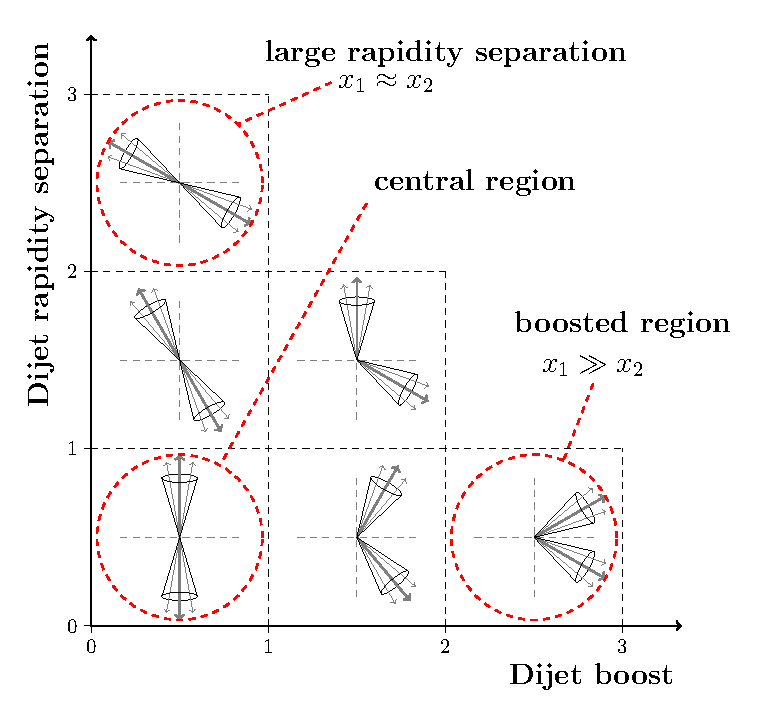
\includegraphics[width=0.5\textwidth]{figures/drawings/ybys_hint.pdf}
\end{SCfigure}

The thesis is structured as follows: In
Chapter~\ref{sec:theoretical_foundations}, the theoretical foundations for dijet
production at hadron colliders are outlined. An overview of the Standard Model
of particle physics with a focus on perturbative QCD is given.  Furthermore, the
relativistic kinematics of dijet production is explained.
Chapter~\ref{sec:experimental_setup} summarizes the experimental setup of the
CMS detector and the measurement and reconstruction of jets. 

The theoretical considerations for the definition of the observables as well as
the accuracy of the NLO calculations are discussed in
Chapter~\ref{sec:theory_predictions}. The measurement of the triple-differential
dijet cross section with the CMS detector is presented in
Chapter~\ref{sec:measurement}. The measurement is scrutinized in a multitude of
studies of the detector and reconstruction efficiencies and a careful
determination of all uncertainties. Furthermore, the cross sections are
corrected for detector effects in an iterative unfolding procedure and are
compared to pQCD calculations at NLO accuracy.

The thesis is rounded off with studies of the PDF sensitivity which are presented in
Chapter~\ref{sec:pdf_constraints}. Constraints on the proton PDFs
are elaborated. Moreover, a simultaneous fit of the PDFs and the strong coupling
is performed to determine the coupling most accurately.

